
\subsubsection{XXX 模型的求解}

基于 1081 个男胎样本(完整案例),采用上述 OLS 线性回归和随机森林两种方法进行求解,关键结果如下。

Y 染色体浓度 与孕周、BMI、年龄、体重等 6 个指标的回归分析显示:线性回归 R² = 0.068(调整 R² = 0.064),5 折 CV R² = 0.055 $\pm$ 0.013;随机森林训练 R² = 0.660,5 折 CV R² = 0.222 $\pm$ 0.046(泛化能力显著优于线性模型)。

OLS 回归系数与显著性检验:孕周 ($\beta$ = 0.513, $p$ < 0.001)、年龄 ($\beta$ = -0.373, $p$ = 0.0002)、体重 ($\beta$ = -0.553, $p$ = 0.002) 三项在 $\alpha = 0.05$ 水平下显著,表明 Y 染色体浓度与孕周呈正相关、与年龄和体重呈负相关。Y 浓度、孕周、BMI 的散点关系与拟合线如图~\ref{fig:q1_scatter} 所示。

\begin{figure}[ht]
  \begin{center}
    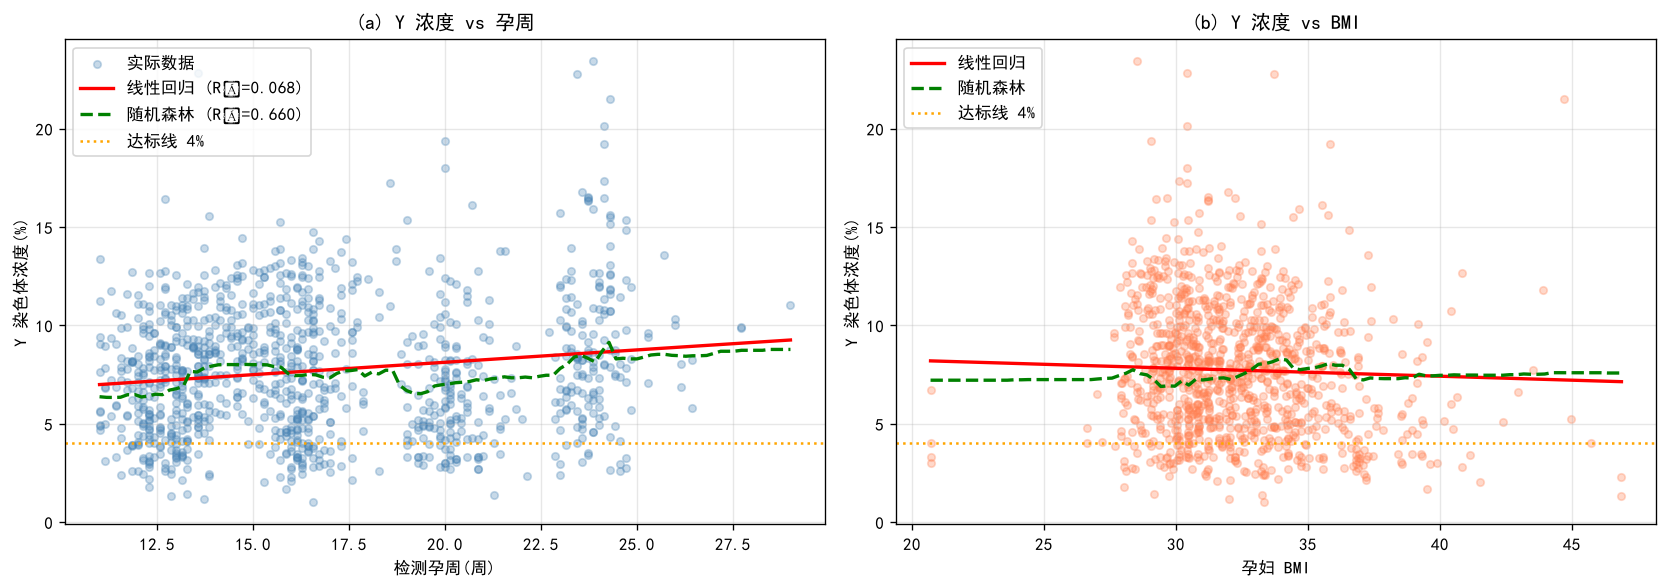
\includegraphics[width=0.85\textwidth]{../求解/问题1/图片/1_Y浓度vs孕周_BMI.png}
    \caption{Y 浓度 vs 孕周(左)与 vs BMI(右)散点 + 拟合线(线性 + RF)}
    \label{fig:q1_scatter}
  \end{center}
\end{figure}

随机森林特征重要性排序为:体重(0.287)> BMI(0.269)> 孕周(0.258)> 年龄(0.186)> IVF(0.000),与 OLS 显著项基本一致,验证了 Y 浓度主要受体重 / BMI / 孕周 / 年龄四因素影响,IVF 妊娠在男胎样本中无变化(图~\ref{fig:q1_imp})。

\begin{figure}[ht]
  \begin{center}
    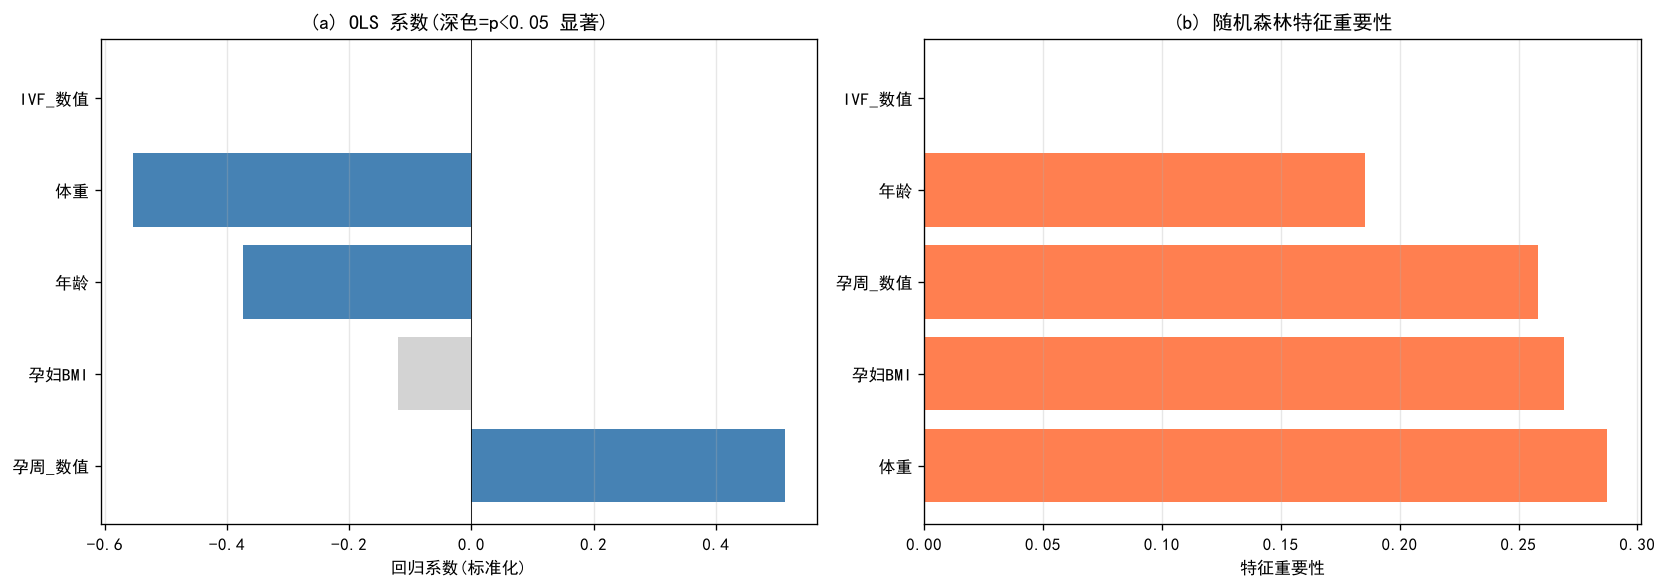
\includegraphics[width=0.85\textwidth]{../求解/问题1/图片/4_系数_特征重要性.png}
    \caption{OLS 标准化系数(深色 = 显著)与随机森林特征重要性}
    \label{fig:q1_imp}
  \end{center}
\end{figure}

5 折交叉验证显示:线性回归 RMSE = 3.24 $\pm$ 0.24,随机森林 RMSE = 2.94 $\pm$ 0.24,提示在 Y 浓度预测任务上随机森林具有显著优势,但 OLS 的可解释性更强。预测值与实际值的散点图如图~\ref{fig:q1_pred} 所示。

\begin{figure}[ht]
  \begin{center}
    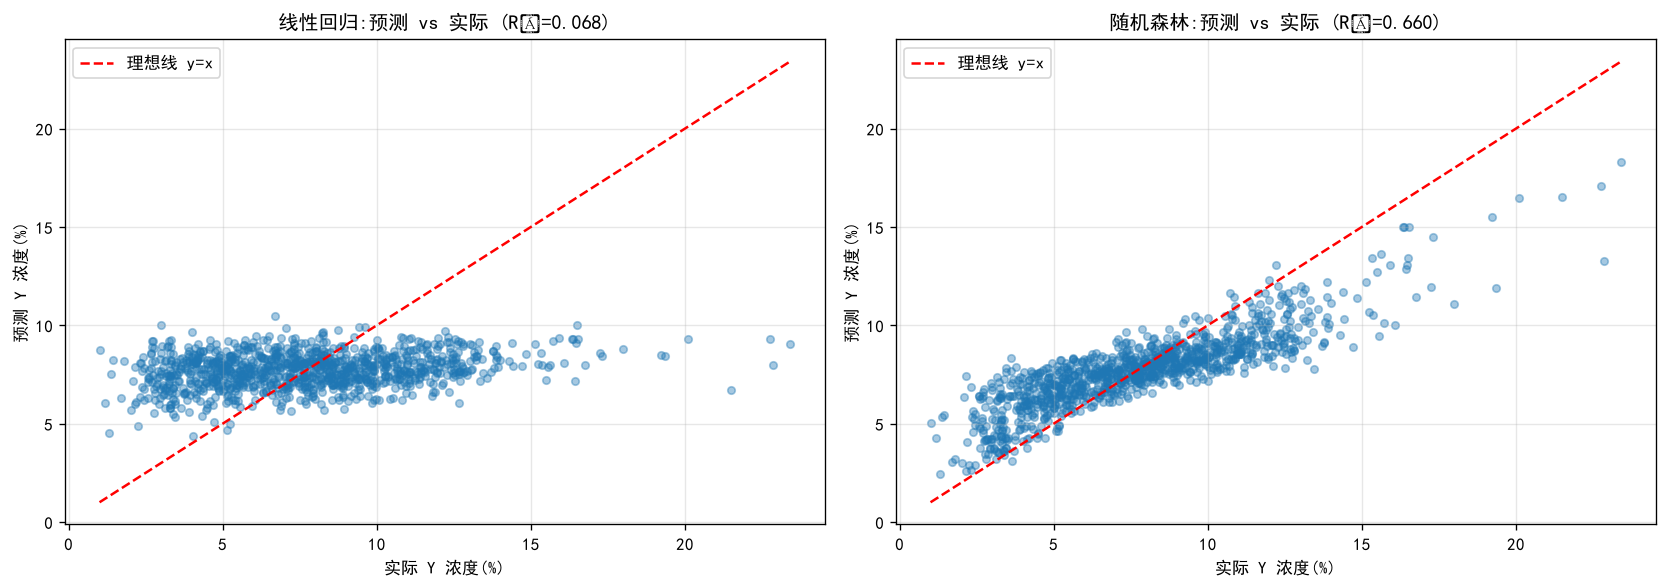
\includegraphics[width=0.85\textwidth]{../求解/问题1/图片/2_预测vs实际.png}
    \caption{预测值 vs 实际值(线性回归与随机森林对比)}
    \label{fig:q1_pred}
  \end{center}
\end{figure}

\begin{longtable}{>{\centering\arraybackslash}p{0.20\textwidth}>{\centering\arraybackslash}p{0.20\textwidth}>{\centering\arraybackslash}p{0.20\textwidth}>{\centering\arraybackslash}p{0.20\textwidth}}
  \caption{问题 1 模型对比}\\
  \toprule
  指标 & 线性回归(OLS) & 随机森林(RF) & 说明 \\
  \midrule
  \endfirsthead
  \caption{问题 1 模型对比(续)}\\
  \toprule
  指标 & 线性回归(OLS) & 随机森林(RF) & 说明 \\
  \midrule
  \endhead
  \bottomrule
  \endfoot
  $R^2$(训练) & 0.068 & 0.660 & 决定系数 \\
  5 折 CV $R^2$ & 0.055 & 0.222 & 泛化能力 \\
  RMSE(训练) & 3.235\% & 1.953\% & 均方根误差 \\
  5 折 CV RMSE & 3.245\% & 2.944\% & 泛化误差 \\
  MAE & 2.620\% & — & 平均绝对误差 \\
\end{longtable}

综上,线性回归可解释孕周(+)、年龄(-)、体重(-) 三因素显著,但 $R^2$ 偏低提示线性假设不足;随机森林精度高但可解释性弱。后续问题 2-3 的最佳时点计算采用问题 1 的随机森林模型作为基准,问题 4 的女胎异常判定使用 OLS 系数作为可解释依据。
